\documentclass{beamer}

\usepackage{Vor2018glærur}

\title{Tölvunarfræði 2}
\subtitle{Vika 7}

\begin{document}

\begin{frame}
\titlepage
\end{frame}

\section{Miðmisseriskönnun}

\begin{frame}{Miðmisseriskönnun}
\begin{center}
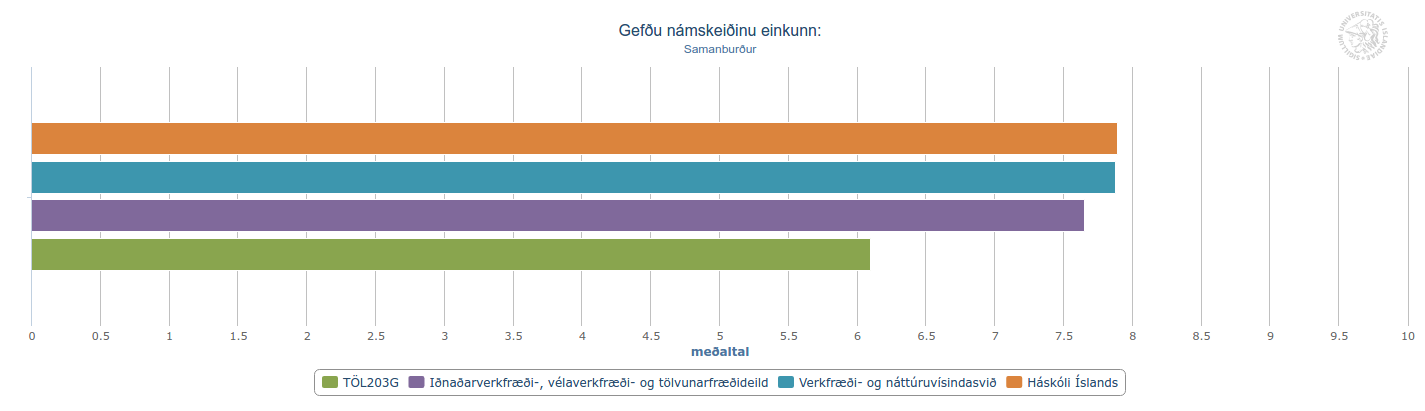
\includegraphics[width=\textwidth]{midmisseriskonnun}
\end{center}
Meðaleinkunn 6.1, 45\% þátttaka
\end{frame}

\begin{frame}{Atriði sem komu fram}
\begin{itemize}
 \item Gott:
 \begin{itemize}
  \item Piazza \pause
 \end{itemize}
 \item Verra:
 \begin{itemize}
  \item \textbf{HEIMADÆMI ALLT OF LÖNG OG ERFIÐ}
  \item Salurinn er ekki nógu góður
  \item Dæmatímar illa nýttir
  \item Fyrirlestrar illa nýttir
 \end{itemize}
 \item Listarnir eru ekki tæmandi, en þessi atriði voru nefnd endurtekið
\end{itemize}
\end{frame}

\begin{frame}{Breytingar}
\begin{itemize}
 \item Heimadæmi verða kerfisbundið einfölduð
 \begin{itemize}
  \item Tvö einföld, tvö eins og þau hafa verið
 \end{itemize}
 \item Dæmatímakennarar sjá um að setja inn nemendalausnir
 \begin{itemize}
  \item Uppfærðir skilmálar á heimadæmablöðum, mikilvægt að lesa!
 \end{itemize}
 \item Meiri töflukennsla í dæmatímum
 \begin{itemize}
  \item Mikilvægt að mæta undirbúin með spurningu!
 \end{itemize}
 \item Við erum stödd í Háskólatorgi, HT-105
 \item Skoðanakönnun um framtíð yfirferðar: \url{https://goo.gl/forms/2IPHR77I2DsfpzHl2}
\end{itemize}
\end{frame}

\section{Yfirlit röðunaraðferða}

\begin{frame}{Myndrænn samanburður}
\begin{itemize}
 \item Valröðun: Glæra 17 á \href{http://algs4.cs.princeton.edu/lectures/21ElementarySorts.pdf}{Elementary sorts}
 \item Innsetningarröðun: Glæra 25 í \href{http://algs4.cs.princeton.edu/lectures/22Mergesort.pdf}{Elementary sorts}
 \item Ofansækin sameiningarröðun: Glæra 9 í \href{http://algs4.cs.princeton.edu/lectures/22Mergesort.pdf}{Merge sort}
 \item Neðansækin sameiningarröðun: Glæra 24 í \href{http://algs4.cs.princeton.edu/lectures/22Mergesort.pdf}{Merge sort}
\end{itemize}
\end{frame}

\section{Quicksort}

\begin{frame}{Quicksort}
\begin{itemize}
 \item Quicksort er skilvirkt og mikið notað röðunarreiknirit
 \begin{itemize}
  \item Hefur verið gríðarlega mikið rannsakað síðan þá
  \item Kostir og gallar reikniritsins eru vel þekktir
  \item Meðal rannsakenda: Robert Sedgewick
 \end{itemize}
\item Quicksort fundið upp af Tony Hoare 1960
 \begin{itemize}
  \item Fann það upp við nám í rússlandi, til að raða orðum 
  \item Hoare er líka þekktur fyrir framlag til formlegra forritunaraðferða og ALGOL forritunarmálsins
 \end{itemize}
\end{itemize}
\end{frame}

\begin{frame}{Lýsing}
\begin{itemize}
 \item Lýsing á quicksort:
 \begin{enumerate}
  \item Veljum safn til að raða og eitthvert stak innan þess til að þjóna sem vendistak \eng{pivot}
  \item Skiptum upp \eng{partition} og endurröðum safninu svo að vendistakið sé á réttum stað, engin stök stærri en vendistakið séu í vinstri hluta þess og engin stök minni en vendistakið séu í hægri hluta þess
  \item Notum quicksort endurkvæmt á hvorn hluta fyrir sig
 \end{enumerate}
 \item Skoðum \texttt{Quick.java} og glæru 15 í \href{http://algs4.cs.princeton.edu/lectures/23Quicksort.pdf}{Quicksort}
\end{itemize}
\end{frame}

\begin{frame}{Skilvirkni}
\begin{itemize}
 \item Besta mögulega tilfelli quicksort - hvert fallskall myndar helmingaskiptingu á safninu
 \begin{itemize}
  \item Besti samanburðarfjölda má lýsa með $C_N = 2C_{N/2} + N$, svo $C_N \sim N \log N$
 \end{itemize}
 \item Ástæða fyrir raunverulegri skilvirkni - meðaltilfellið er litlu verra en það besta
 \begin{itemize}
  \item Ekki nema 39\% fleiri samanburðir í ``meðaltilfellinu''
  \item Má sanna með tölfræðilegum aðferðum
 \end{itemize}
 \item Í versta tilfellinu - öll stökin lenda á sömu hlið við vendistakið
 \begin{itemize}
  \item $\sim \frac{N^2}{2}$ samanburðir, en þetta tilvik má venjulega forðast
 \end{itemize}
 \item Oft betra en sameiningarröðun vegna fárra skiptinga og eiginleika raunverulegra örgjörva
 \item Skoðum \texttt{SortCompare.java}
\end{itemize}
\end{frame}

\begin{frame}{Endurbætur}
\begin{itemize}
 \item Hægt er að fá meiri hraða úr quicksort með smábreytingum frá \texttt{Quick.java}
 \begin{itemize}
  \item Skipta yfir í innsetningarröðun á smáfylkjum
  \item Meðhöndla jafn stór stök sérstaklega
  \begin{itemize}
   \item Sjá \texttt{Quick3way.java}
  \end{itemize}
  \item Gott val á vendistaki - t.d. Median-of-3
 \end{itemize}
\end{itemize}
\end{frame}

\begin{frame}{Hvaða röðunarreiknirit?}
Skoðum glæru 48 í \href{http://algs4.cs.princeton.edu/lectures/23Quicksort.pdf}{Quicksort}.
\end{frame}

\section{Forgangsbiðraðir}

\begin{frame}{Forgangsbiðröð}
\begin{itemize}
 \item Forgangsbiðröð (e. \emph{priority queue}) er hugræn gagnagerð
 \item Almennari gagnagerð en hlaðar og biðraðir, sem við höfum séð áður
 \begin{itemize}
  \item Í hlaða: Eyðing framkvæmd á því staki sem styst hefur verið á hlaðanum
  \item Í biðröð: Eyðing framkvæmd á því staki sem lengst hefur verið í biðröðinni
  \item Í forgangsbiðröð: Eyðing framkvæmd á því staki sem hefur hæsta gildið
 \end{itemize}
\end{itemize}
\end{frame}

\begin{frame}{API}
Möguleg skil fyrir forgangsbiðröð:
\begin{center}
\begin{tabularx}{\textwidth}{rlX}
\toprule
\multicolumn{3}{c}{\texttt{public class MaxPQ<Key>}}\\
\midrule
-&\texttt{MaxPQ()}& Smiður, býr til tóma forgangsbiðröð\\
\texttt{void}&\texttt{insert(Key v)}&Bæta stakinu \texttt{key} við f-biðröðina\\
\texttt{Key}&\texttt{max()}&Skila stærsta stakinu í biðröðinni\\
\texttt{Key}&\texttt{delMax()}&Fjarlægja og skila stærsta stakinu í biðröðinni\\
\texttt{boolean}&\texttt{isEmpty()}&Er forgangsbiðröðin tóm?\\
\texttt{int}&\texttt{size()}&Fjöldi hluta í forgangsbiðröðinni\\
\bottomrule
\end{tabularx}
\end{center}
Aths: Gætum allt eins skilgreint ``minimum priority queue''. \texttt{Key} þarf að vera samanburðarhæfur.
\end{frame}

\begin{frame}{Skilvirkni forgangsbiðraða}
Aðgerðir á forgangsbiðröð af lengd $N$ þurfa tíma sem er háður undirliggjandi gagnagrind
\begin{center}
\begin{tabular}{lcc}
\toprule
Gagnagrind&Innsetning&Fjarlægja hæsta\\
\midrule
Raðað fylki&$N$&1\\
Óraðað fylki&1&$N$\\
Hrúga&$\log N$&$\log N$\\
Einhyrningur\footnote{Einhyrningar eru ekki til}&1&1\\
\bottomrule
\end{tabular}
\end{center}
Það að nota óraðað fylki er ``löt'' aðferðafræði, það að nota raðað fylki ``áköf'' aðferðafræði.
\end{frame}

\section{Hrúgur}

\begin{frame}{Hrúgur}
Hrúga \eng{heap} er tré sem uppfyllir hrúguskilyrði \eng{heap property}. Við notum fylki til að geyma hrúgur.

Skoðum glærur 16-17, 20-23 í \href{http://algs4.cs.princeton.edu/lectures/24PriorityQueues.pdf}{PriorityQueues}.
\end{frame}

\begin{frame}{Tími}
\begin{itemize}
 \item Athugum - um fullskipuð tré er að ræða
 \item Innsetning og eyðing felur í sér færslu á milli hæða í trénu
 \item Fjöldi aðgerða takmarkast af hæð trésins
 \begin{itemize}
  \item Hæð fullskipaðs trés með $N$ hnútum er $\lfloor \log_2 n \rfloor$
 \end{itemize}
 \item Praktísk vandræði - langt á milli staka, hentar skyndiminni örgjörva illa
\end{itemize}
\end{frame}

\begin{frame}{Þessi glærupakki}
Tengill á fyrirlestraræfingu: \url{https://goo.gl/forms/b4uyD6Z17qfsevas1}
\vspace{1cm}

\texttt{SortCompare.java} má finna á \href{https://github.com/Ernir/kennsluefni/tree/master/T2/Code/w7}{Github}. 

Kóða fyrir algs4 reiknirit má finna á \url{http://algs4.cs.princeton.edu/code/}
\end{frame}


\end{document}
